\chapter{Implementacja}
\label{cha:implementacja}

%---------------------------------------------------------------------------

\section{Zestaw narzędzi i technologii}
\label{sec:zestawNardzedziITechnologii}

Aplikacja została zaimplementowana z myślą o telefonie komórkowym z systemem operacyjnym Android. Najstarszą wersją systemu, jaką wspiera \textit{HowAreYou} jest Lollipop (minimalne SKD zostało ustawione na 22). 

Wraz z~potrzebą akwizycji dużej ilości różnego rodzaju danych z~sensorów urządzenia mobilnego pojawiła się konieczność realizacji tej akwizycji. Zdecydowano się pominąć własną implementację tego mechanizmu wykorzystując szeroki wachlarz możliwości jaki daje jeden z~otwartoźródłowych frameworków. Ostatecznie wybór padł na framework \textit{AWARE}. Rozwiązanie realizujące różne metody mediacji wiedzy zostało więc stworzone jako plugin \textit{HowAreYou} - nieoficjalne rozszerzenie \textit{AWARE}.

Implementacja pluginu została zrealizowana w~języku Java, rekomendowanym przez twórców frameworka \textit{AWARE}\cite{AwareFramework}. Środowiskiem wykorzystanym w~celu realizacji zadania było Android Studio. Do kontroli wersji wykorzystano narzędzie git, do przechowywania kodu źródłowego -- platformę github: \url{https://github.com/filipbiernat/HowAreYou_plugin}.

%---------------------------------------------------------------------------

\section{Model HMR}
\label{sec:modelHmr2}

\subsection{Konstruowanie modelu wnioskującego}

Do tworzenia pliku \textit{model.hmr} wykorzystana została aplikacja webowa \textit{HeaKatE Web Editor} (w~skrócie \textit{HWEd}). \textit{HWEd} jest edytorem online (stworzonym z~wykorzystaniem środowiska \textit{node.js}) służącym do tworzenia i edytowania modeli, które później wykorzystywane są przez silnik wnioskujący \textit{HeaRTDroid} \cite{heartdroid}. Zawarty w~nim parser przetwarza reguły \textit{XTT2} na czytelne dla użytkownika zestawy połączonych ze sobą tabel, a następnie po wybraniu opcji \textit{Export} przekształca tablice w~plik HMR z~regułami \textit{XTT2} \cite{heartdroid}.

Samo \textit{XTT2} jest formalizmem reprezentacji wiedzy stworzonym z~myślą o regułach. Służy algebraicznej i logicznej specyfikacji reguł pozwalając na zwięzły, przejrzysty i efektywny sposób wizualnej reprezentacji wiedzy. W odróżnieniu od tradycyjnych systemów pozwala wykorzystanie ,,płaskiego'' (jednoopoziomowego) zestawu reguł. Wprowadza tablice, wykorzystywane do reprezentowania zestawów reguł mających podobrą strukturę, oraz połączenia między tablicami. Struktura zestawów tabel przypomina drzewa decyzyjne \cite{AiWikiHekate}.

Podczas opracowywania modelu wykorzystane zostało również narzędzie \textit{HeaRTDroid Query Notation} (w skrócie \textit{HaQuNa}). \textit{HaQuNa} jest prostym językiem, który może być wykorzystywany w~interaktywnej powłoce. Zestaw poleceń linii komend umożliwia wczytywanie, modyfikację oraz uruchamianie modeli HMR\cite{heartdroid}. Przy implementacji \textit{HowAreYou} \textit{HaQuNa} była wykorzystywana do weryfikacji poprawności tworzonego modelu.

Należy jeszcze podkreślić, że model HMR został architektonicznie oddzielony od implementacji aplikacji. Dzięki zastosowaniu tego rozwiązania, plugin \textit{HowAreYou} nie musi być powiązany z~obecnie zaimplementowanym domyślnym modelem. Ekspert domenowy, który nie musi być nawet osobą techniczną, może bez trudu z~wykorzystaniem edytora online stworzyć nowy zestaw reguł \textit{XTT2} i zastąpić w~strukturze projektu plik \textit{model.hmr}.

\subsection{Zaawansowany model wnioskujący}

Celem realizacji zaawansowanego modelu wnioskującego było opracowanie modelu, z~pomocą którego zostaną wybrane jak najlepszy moment i sposób na zapytanie użytkownika o jego samopoczucie. Możliwe jest zapytanie niejawne poprzez wykonanie i przetworzenie fotografii lub zapytanie jawne - o kolor lub bezpośrednio o emocje.

W procesie wnioskowania brane są pod uwagę czynniki takie jak czas, który upłynął od ostatniego zapytania, korzystanie z~nawigacji samochodowej, wykonywanie połączenia telefonicznego, oglądanie filmów, czy wykonywanie ruchu. Uwzględniane są też wyniki analizy fotografii oraz wiedza, czy w~danej chwili użytkownik korzysta z~ekranu telefonu.

W sekcji omówiono kolejno strukturę zaimplementowanego modelu oraz poszczególne elementy stworzonego rozwiązania -- tabele, na podstawie których silnik wnioskujący podejmuje decyzje.

\subsubsection{Realizacja zaawansowanego modelu wnioskującego}

Poniższe obrazy przedstawiają widok modelu HMR w~edytorze \textit{HWEd}. Model został skonstruowany jako zestaw tabel, które zależąc od informacji z~aplikacji oraz od siebie nawzajem realizują reguły decyzyjne. Decyzja z~jednej tabeli ma bezpośreni wpływ na działanie kolejnej. Ostatecznie zgodnie z~wynikiem z~ostatniej tabeli \textit{howareyouAction} plugin \textit{HowAreYou} podejmuje określoną akcję. W kolejnej części rozdziału omawiane zostają krok po kroku zasady działania poszczególnych tabel poniższego modelu.

\begin{figure}[H]
	\centering
	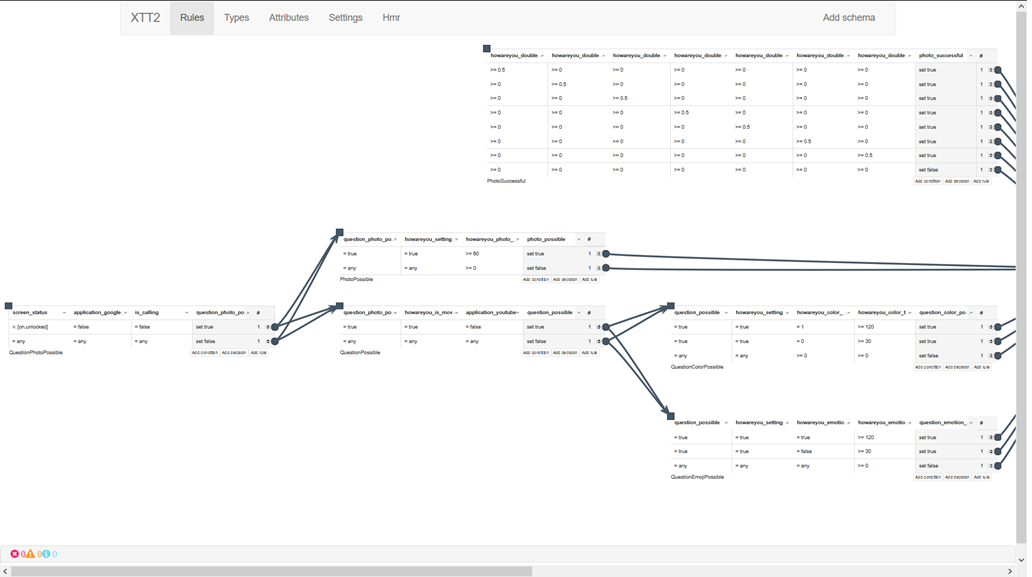
\includegraphics[scale=0.75]{rozdzial4/HMR_advancedModelPart1.png}
	\caption{Zaawansowany model wnioskujący: część 1.}
\end{figure}

\begin{figure}[H]
	\centering
	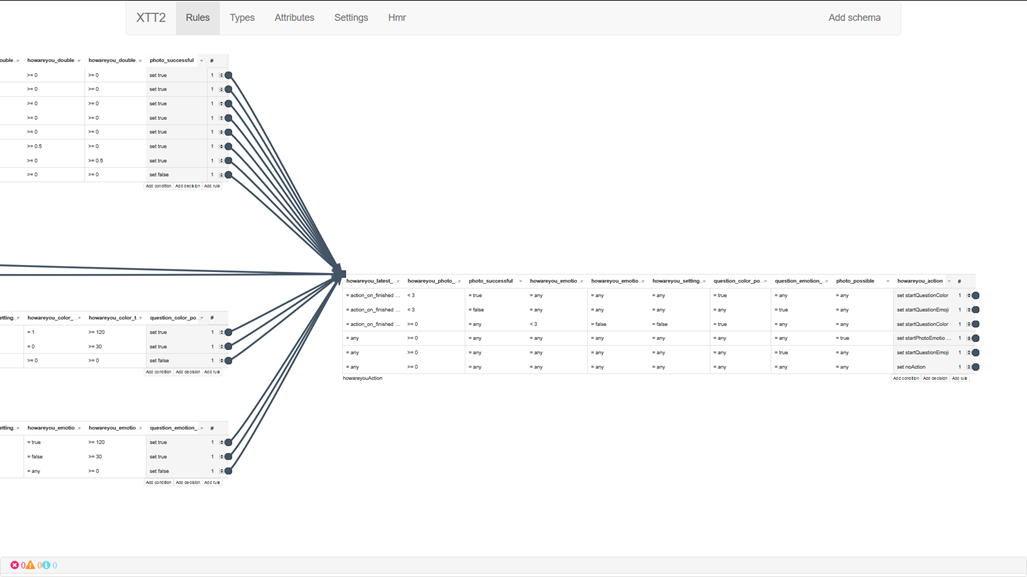
\includegraphics[scale=0.75]{rozdzial4/HMR_advancedModelPart2.png}
	\caption{Zaawansowany model wnioskujący: część 2.}
\end{figure}


\subsubsection{Tabela QuestionPhotoPossible}

Tabela zwraca prawdę, jeżeli spełnione są wspólne warunki konieczne do zapytania użytkownika lub wykonania zdjęcia.

Żeby uruchomić pytanie lub zrobić zdjęcie ekran telefonu musi być aktywny, telefon nie może prowadzić nawigacji, ani wykonywać połączenia.

\begin{figure}[H]
	\centering
	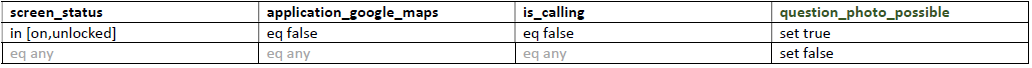
\includegraphics[scale=0.75]{rozdzial4/HMR_QuestionPhotoPossible.png}
	\caption{Zaawansowany model wnioskujący: tabela QuestionPhotoPossible.}
\end{figure}


\subsubsection{Tabela PhotoPossible}

Tabela zwraca prawdę, jeżeli spełnione są warunki konieczne do wykonania zdjęcia.

Żeby zrobić zdjęcie telefon musi spełniać warunki konieczne wspólne dla zdjęcia i pytania. Dodatkowo opcja wykonywania zdjęć musi być uruchomiona i czas, jaki upłynął od ostatniego zdjęcia, musi być większy lub równy 60 minut.

\begin{figure}[H]
	\centering
	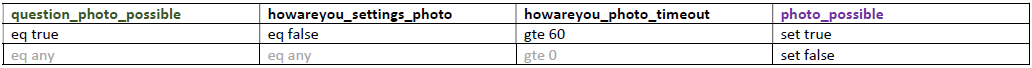
\includegraphics[scale=0.75]{rozdzial4/HMR_PhotoPossible.png}
	\caption{Zaawansowany model wnioskujący: tabela PhotoPossible.}
\end{figure}


\subsubsection{Tabela QuestionPossible}

Tabela zwraca prawdę, jeżeli spełnione są warunki konieczne do zapytania użytkownika.

Żeby uruchomić pytanie telefon musi spełniać warunki konieczne wspólne dla zdjęcia i pytania. Dodatkowo musi znajdować się w~ruchu (jeżeli jest w~bezruchu, najprawdopodobniej jest odłożony) i nie może być uruchomiona aplikacja do oglądania filmów. 

\begin{figure}[H]
	\centering
	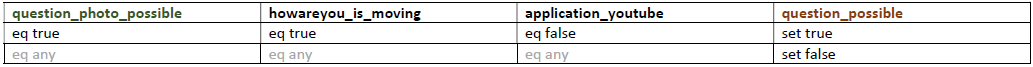
\includegraphics[scale=0.75]{rozdzial4/HMR_QuestionPossible.png}
	\caption{Zaawansowany model wnioskujący: tabela QuestionPossible.}
\end{figure}


\subsubsection{Tabela QuestionColorPossible}

Tabela zwraca prawdę, jeżeli spełnione są warunki konieczne do zapytania użytkownika o kolor.

Żeby uruchomić pytanie o kolor telefon musi spełniać warunki konieczne do zadania pytania. Dodatkowo ustawienia pluginu muszą pozwalać zapytać o kolor. Jeżeli ostatnie pytanie o kolor było odrzucone, kolejne pytanie może być zadane po 120 minutach. Jeżeli nie było odrzucone – po 30 minutach.

\begin{figure}[H]
	\centering
	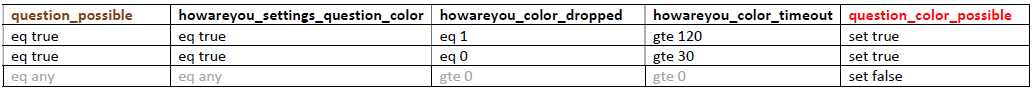
\includegraphics[scale=0.75]{rozdzial4/HMR_QuestionColorPossible.png}
	\caption{Zaawansowany model wnioskujący: tabela QuestionColorPossible.}
\end{figure}


\subsubsection{Tabela QuestionEmojiPossible}

Tabela zwraca prawdę, jeżeli spełnione są warunki konieczne do zapytania użytkownika o emocje.

Żeby uruchomić pytanie o emocje telefon musi spełniać warunki konieczne do zadania pytania. Dodatkowo ustawienia pluginu muszą pozwalać zapytać o emocje. Jeżeli ostatnie pytanie o emocje było odrzucone, kolejne pytanie może być zadane po 120 minutach. Jeżeli nie było odrzucone – po 30 minutach.

\begin{figure}[H]
	\centering
	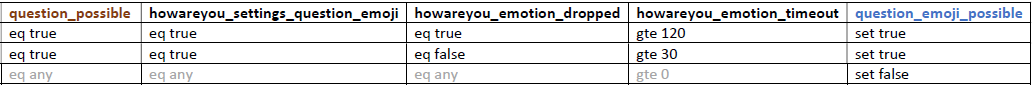
\includegraphics[scale=0.75]{rozdzial4/HMR_QuestionEmojiPossible.png}
	\caption{Zaawansowany model wnioskujący: tabela QuestionEmojiPossible.}
\end{figure}


\subsubsection{Tabela PhotoSuccessful}

Tabela zwraca prawdę, jeżeli najnowsze zdjęcie w~bazie danych uznaje się za udane.

Żeby uznać zdjęcie za udane wystarczy, że wartość prawdopodobieństwa jednej z~wykrytych emocji (za wyjątkiem emocji \textit{neutral}) jest większa niż próg (który obecnie wynosi 50 procent pewności).

\begin{figure}[H]
	\centering
	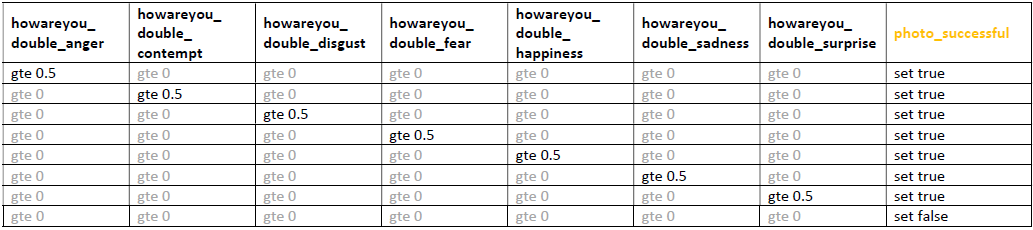
\includegraphics[scale=0.75]{rozdzial4/HMR_PhotoSuccessful.png}
	\caption{Zaawansowany model wnioskujący: tabela PhotoSuccessful.}
\end{figure}


\subsubsection{Tabela howareyouAction}

Tabela zwraca prawdę, jeżeli najnowsze zdjęcie w~bazie danych uznaje się za udane. 
\begin{enumerate}
	\item Jeżeli ostatnią akcją jaką plugin wykonał było zdjęcie i to zdjęcie było niedawno (mniej niż 3 minuty temu) i to zdjęcie było udane, to telefon zapyta o kolor, jeżeli spełnione są warunki do zapytania o kolor.
	\item Jeżeli ostatnią akcją jaką plugin wykonał było zdjęcie i to zdjęcie było niedawno (mniej niż 3 minuty temu), ale nie było udane, to telefon zapyta o emocje, jeżeli spełnione są warunki do zapytania o emocje.
	\item Jeżeli ostatnią akcją jaką plugin wykonał było pytanie o emocje i to pytanie o emocje było niedawno (mniej niż 3 minuty temu) i użytkownik odpowiedział na to pytanie, to telefon zapyta o kolor, jeżeli spełnione są warunki do zapytania o kolor. Ta reguła (de facto dwa pytania jedno po drugim) wykona się tylko wtedy, gdy użytkownik w~ustawieniach wyłączył wykonywanie zdjęć. 
	\item Jeżeli jest możliwe zrobienie zdjęcia, to telefon wykona zdjęcie. 
	\item Jeżeli nie jest możliwe zrobienie zdjęcia, to telefon zapyta o emocje, jeżeli spełnione są warunki do zapytania o emocje.
	\item Jeżeli żadna z~akcji nie jest możliwa, telefon nie wykona akcji.
\end{enumerate}

\begin{figure}[H]
	\centering
	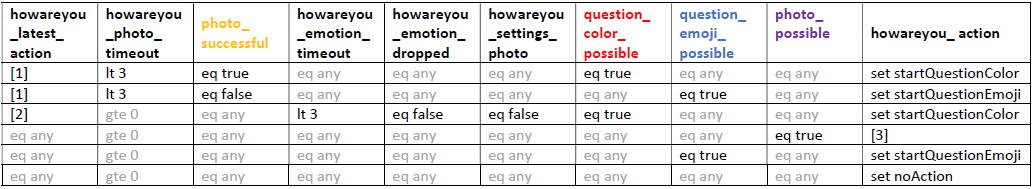
\includegraphics[scale=0.75]{rozdzial4/HMR_howareyouAction.png}
	\caption{Zaawansowany model wnioskujący: tabela howareyouAction.}
\end{figure}


\subsubsection{Obserwowanie reguł wnioskujących}

Działanie systemu wnioskującego wykorzystującego zaawansowany model wnioskujący można obserwować na bieżąco z~wykorzystaniem trybu debugowego. Po wybraniu opcji \textit{Otwórz log z~ostatniego wnioskowania} w~ustawieniach pluginu \textit{HowAreYou}, oczom użytkownika ukaże się okno ze szczegółowym opisem elementów wnioskowania: tabel, reguł i decyzji, jakie zostały podjęte.

\begin{figure}[H]
	\centering
	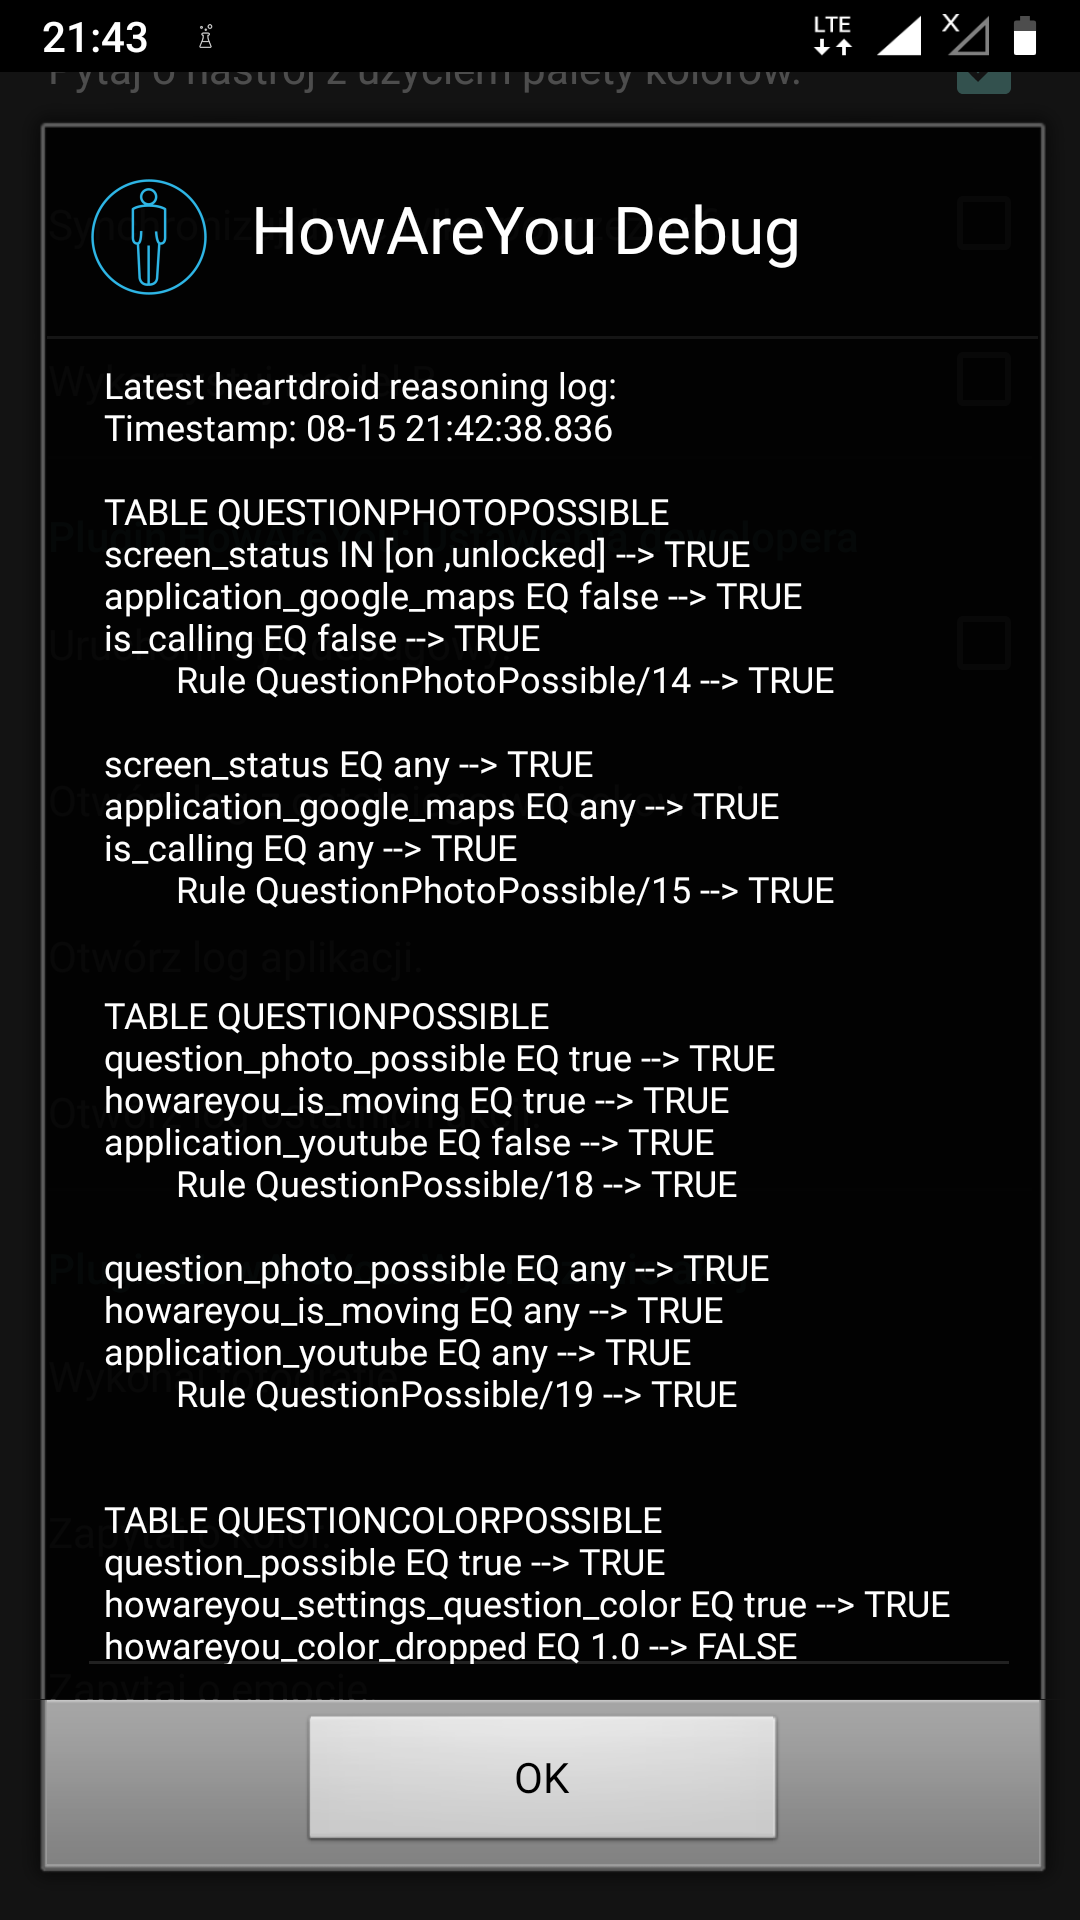
\includegraphics[scale=0.15]{rozdzial4/HMR_screenshots_A.png}
	\caption{Tryb debugowy: widok z~fragmentem loga z~wnioskowania HMR.}
\end{figure}



\subsection{Uproszczony model wnioskujący}

W celach badawczych został stworzony również model uproszczony. Dzięki niemu osoba przeprowadzająca badanie jest w~stanie porównać, jaki wpływ na odbieranie przez uczestnika uciążliwości badania ma złożoność samego modelu. Model prosty został stworzony w~kontraście do pierwszego modelu. Sam model wykorzystuje tylko 2 czynniki: wiedzę czy ekran jest urządzenia włączony oraz czas od ostatniego zapytania. Model symuluje prosty i toporny system odpytywania użytkownika. 

W sekcji omówiono kolejno założenia i przyczyny powstania drugiego modelu oraz sposób w jaki został on skonstruowany.

\subsubsection{Realizacja uproszczonego modelu wnioskującego}

Zdecydowaną zaletą \textit{HowAreYou} jest fakt, iż w~celach porównawczych nie było niezbędne tworzenie dodatkowej aplikacji, która odpytywałaby użytkownika w~sposób uproszczony, ani nawet modyfikacja kodu źródłowego aplikacji. Jedyną potrzebną czynnością była zmiana samego modelu HMR. Model uproszczony można aktywować w~ustawieniach aplikacji. Można również zainstalować plugin \textit{HowAreYou} bezpośrednio z~modelem uproszczonym. Podczas pobierania pliku instalatora należy wybrać wersję B (\textit{patrz: dodatek A}).


\subsubsection{Tabela howareyouAction}

Tabela zwraca prawdę, jeżeli najnowsze zdjęcie w~bazie danych uznaje się za udane. 
\begin{enumerate}
	\item Jeżeli ekran urządzenia jest aktywny i od ostatniego zapytania minęło co najmniej 60 minut, aplikacja zapyta użytkownika o emocje.
	\item Jeżeli któryś z~powyższych warunków nie jest spełniony, telefon nie wykona żanej akcji.
\end{enumerate}

\begin{figure}[H]
	\centering
	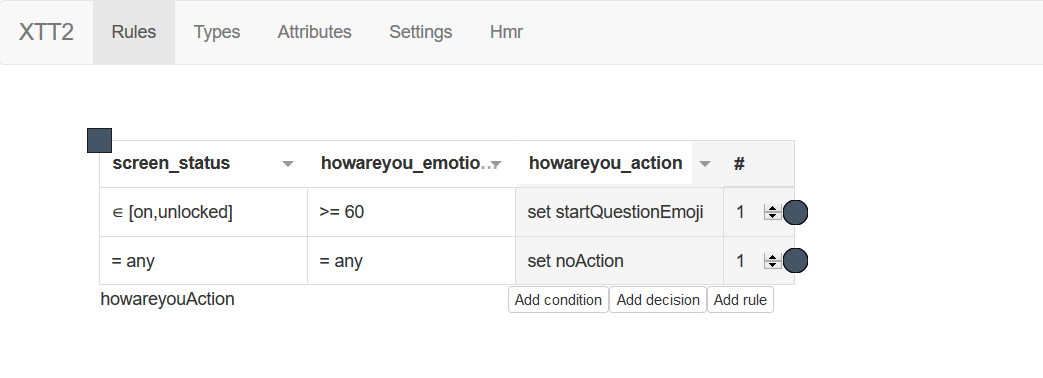
\includegraphics[scale=0.8]{rozdzial4/HMR_basic.png}
	\caption{Uproszczony model wnioskujący: tabela howareyouAction.}
\end{figure}

\subsubsection{Obserwowanie reguł wnioskujących}

Podobnie jak w~przypadku zaawansowanego modelu, działanie systemu wnioskującego wykorzystującego uproszczony model można obserwować na bieżąco z~wykorzystaniem trybu debugowego. Tutaj jednak log z~wnioskowania jest znacznie krótszy - do tego stopnia, że obejmuje tylko jedną tabelę i tylko dwie reguły.

\begin{figure}[H]
	\centering
	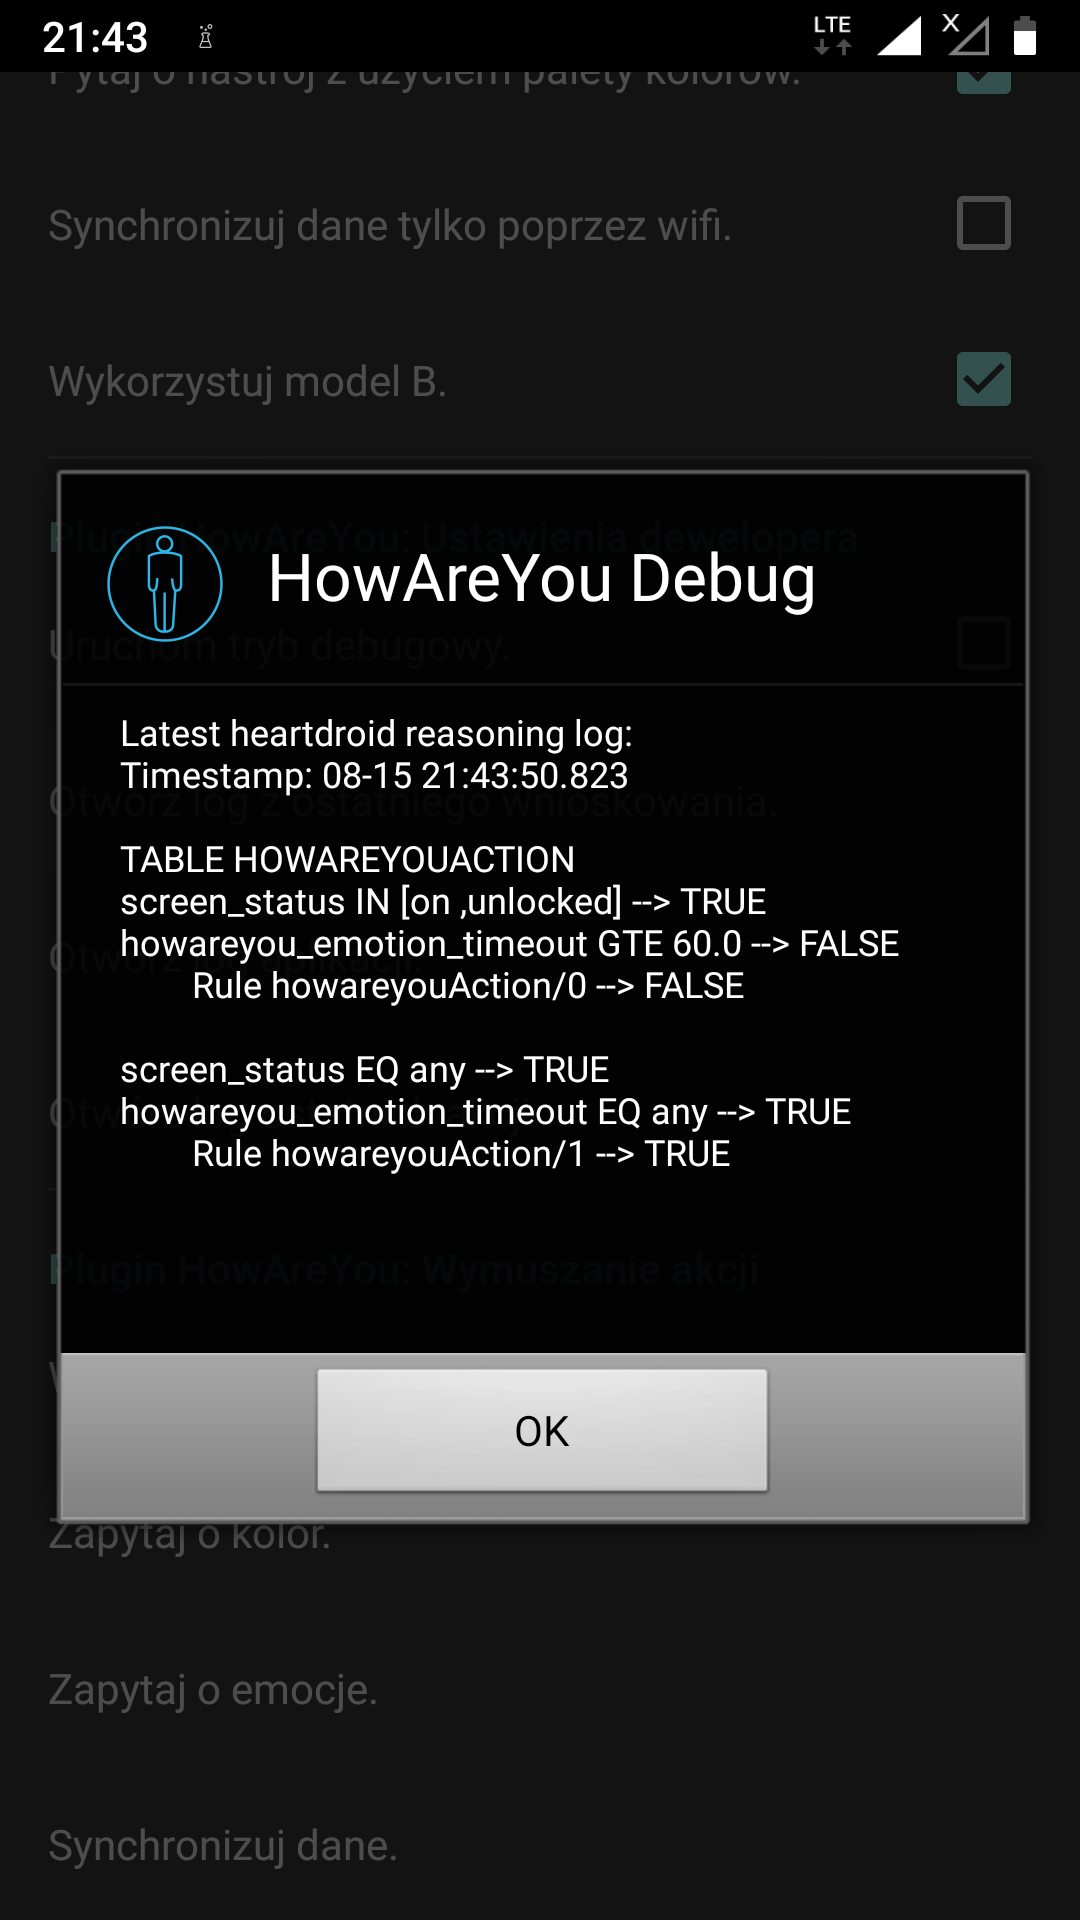
\includegraphics[scale=0.15]{rozdzial4/HMR_screenshots_B.png}
	\caption{Tryb debugowy: widok z~loga z~wnioskowania HMR z~modelem uproszczonym.}
\end{figure}

%---------------------------------------------------------------------------

\section{Pakiet \textit{HeaRT-AWARE}}
\label{sec:pakietHeartAware2}

Jak już wspomniano w~poprzednim rozdziale, zadaniem pakietu \textit{agh.heart} było zintegrowanie ze sobą frameworka \textit{AWARE} i silnika wnioskującego \textit{HeaRTDroid}. Zostało ono zaprojektowane przez autora pakietu w~formie trzech pomniejszych specjalistycznych pakietów: \textit{actions}, \textit{observers} i \textit{callbacks}\cite{heartaware}.

\subsection{Pakiet \textit{agh.heart.actions}}

W pluginie \textit{HowAreYou} zrezygnowano z~dostępnych początkowo w~pakiecie akcji \textit{DisableBlueTooth} (ang. wyłącz Bluetooth) i \textit{EnableBlueTooth} (ang. włącz Bluetooth). Przy realizacji aplikacji monitorującej nastrój użytkownika nie było potrzeby wykorzystywania tego typu akcji. W zamian zaimplementowano akcje związane ze specyfiką zadania:

\begin{itemize}
	\item \textit{HowAreYou\_StartPhotoEmotionRecognition} -- uruchom usługę odpowiedzialną za rozpoznawanie emocji użytkownika na podstawie fotografii.
	\item \textit{HowAreYou\_StartQuestionEmoji} -- uruchom aktywność odpowiedzialną za zapytanie użytkownika o nastrój z~wykorzystaniem widoku emotikon.
	\item \textit{HowAreYou\_StartQuestionColor} -- uruchom aktywność odpowiedzialną za zapytanie użytkownika o nastrój z~wykorzystaniem widoku kolorów.
\end{itemize}

Każda z~powyższych akcji przesyła wiadomość broadcastową do PluginManagera w~pakiecie \textit{com.aware.plugin.howareyou}. PluginManager uruchamia następnie zaplanowaną aktywność lub usługę. 

Aby uprościć rozwiązanie, zaimplementowano również klasę bazową \textit{HowAreYou\_Action}, z~której korzystają powyższe klasy. Dzięki takiemu rozwiązaniu, jeżeli w~przyszłości pojawiłaby się potrzeba uwzględnienia w~modelu nowej akcji dołączonej do PluginManagera, dołączenie jej do zbioru \textit{actions} powinno być bardzo proste.


\subsection{Pakiet \textit{agh.heart.observers}}

W swojej początkowej formie Pakiet \textit{HeaRT-AWARE} dostarczał użytkownikowi trzy różne klasy obserwatora: \textit{Accelerometer}, \textit{Location} i \textit{Screen}. 

Na potrzeby niniejszej pracy zaimplementowano jeszcze jedną dodatkową klasę \textit{HowAreYou}. Pozwala ona silnikowi wnioskującemu reagować na sytuacje, kiedy użytkownik udzieli odpowiedzi na pytanie (lub odrzuci pytanie wybierając opcję \textit{Nie teraz}), czy też na sytuację, kiedy zostanie wykonana fotografia i zewnętrzne API zwróci wyniki rozpoznawania emocji. W tym przypadku silnik wnioskujący może na bieżąco reagować na te wyniki podejmując decyzję, czy na przykład zapytać dodatkowo o kolor (jeżeli wiemy, co obecnie czuje użytkownik) lub o emocje (jeżeli nie udało ich się rozpoznać automatycznie). 

Nowa klasa ma postać \textit{BroadcastReceivera}, który reaguje na akcje:
\begin{itemize}
	\item \textit{ACTION\_ON\_FINISHED\_QUESTION\_COLOR} -- zakończono zapytanie użytkownika o kolor,
	\item \textit{ACTION\_ON\_FINISHED\_QUESTION\_EMOJI} -- zakończono zapytanie użytkownika bezpośrednio o emocje,
	\item \textit{ACTION\_ON\_FINISHED\_PHOTO\_EMOTION\_RECOGNITION} -- zakończono (z powodzeniem lub nie) proces rozpoznawania emocji użytkownika z~wykorzystaniem kamery telefonu.
\end{itemize}

W modelu HMR dostępnym w~ramach \textit{HowAreYou} zrezygnowano z~wykorzystywania \textit{observers}: \textit{Accelerometer} oraz \textit{Location}. Pozostałe dwa wystarczająco dobrze radzą sobie z~uruchamianiem wnioskowania. Kluczowy jest tutaj obserwator ekranu, który daje znać, czy użytkownik korzysta z~telefonu. Wspomaga go nowy obserwator z~akcjami specyficznymi dla bieżącego rozszerzenia. 

Jeżeli chodzi o dane z~akcelerometru, kłopotliwe może okazać się ich przetwarzanie i filtrowanie -- mamy tutaj do czynienia z~ogromną ilością ,,surowych'' danych. W przypadku danych z~lokalizacji, ciężko wyobrazić sobie dla nich zastosowanie jako dla czynnika uruchamiającego wnioskowanie w~tym konkretnym przypadku. W innym przypadku wiązałoby się to pewnie ze stworzeniem złożonych map obszarów, gdzie po przekroczeniu pewnej granicy, wnioskowanie może zostać uruchomione. Nic nie stoi jednak na przeszkodzie, żeby w~dalszych pracach nad \textit{HowAreYou} powrócić do obecnie pominiętych \textit{observers}.


\subsection{Pakiet \textit{agh.heart.callbacks}}

Ostatnim z~kluczowych elementów przy wnioskowaniu są tzw. \textit{callbacks}, czyli wywołania, które pozwalają mechanizmom wnioskującym na dostęp do parametrów zewnętrzych. Początkowo dysponowaliśmy trzema takimi wywołaniami -- dla żyroskopu (\textit{Gyroscope}), lokalizacji (\textit{Location}) i ekranu urządzenia (\textit{Screen}). Konieczne było jednak opracowanie kolejnych \textit{callbacks}. Im większa ich liczba -- tym dokładniejszy model HMR można skonstruować. 

W pierwszej kolejności zaimplementowano nowe klasy bazowe upraszczające strukturę pakietu. Dzięki zastosowaniu takich ogólnych \textit{callbacks}, uzyskano znacznie łatwiejszą możliwość rozbudowy o kolejne czynniki zewnętrzne.
\begin{itemize}
	\item \textit{GenericDbCallback} -- klasa opakowuje wszystkie funkcjonalności, jakie potrzebne są do pozyskania odpowiednich informacji z~bazy danych. Klasa dziedzicząca po \textit{GenericDbCallback} musi jedynie wyspecyfikować parametry dostępu do bazy danych SQLite takie jak URI i lista kolumn.
	
	\item \textit{Application\_Generic} -- wykorzystuje sensor \textit{AWARE} \textit{Applications\_Foreground}. Po pobraniu informacji z~bazy danych sensora porównuje nazwę zdefiniowanego pakietu z~zapisanym w~podklasie pakietem konkretnej aplikacji. Zwraca 1, jeżeli aktualnie wykorzystywaną aplikacją jest ta zdefiniowana w~podklasie, w~przeciwnym przypadku zwraca 0.
	
	\item \textit{HowAreYou\_Generic} -- początkowo klasa została stworzona z~myślą o wywołaniach charakterystycznych dla konkretnego pluginu. Z czasem znalazła zastosowanie również dla wykorzystywania klasycznych tablic frameworka \textit{AWARE}. Cechą charakterystyczną jest dodatkowa kolumna "\textit{*\_timeout}". Dzięki niej silnik wnioskujący otrzymuje informację jak dawno miało miejsce wydarzenie, do którego się odwołuje. \textit{Timeout} mierzony jest jako różnica pomiędzy bieżącym czasem systemowym oraz czasem zdarzenia zapisanym w~bazie danych (w kolumnie \textit{timestamp}) i jest wyrażony w~minutach.
\end{itemize}

Lista nowo-dodanych wywołań ma się następująco: 

\begin{itemize}
	\item \textit{Application\_Facebook} -- informuje silnik czy aktualnie uruchomiona jest aplikacja \textit{Facebook}.
	
	\item \textit{Application\_GoogleMaps} -- informuje silnik czy aktualnie uruchomiona jest nawigacja.
	
	\item \textit{Application\_YouTube} -- informuje silnik czy użytkownik ogląda filmy w~aplikacji \textit{YouTube}.
	
	\item \textit{Communication} -- informuje silnik czy obecnie trwa połączenie telefoniczne. Wywołanie nie wykorzystuje bazy danych, w~zamian na obiekcie \textit{CommunicationObserver} uruchamiana jest metoda \textit{isCalling}. W ten sposób wykorzystany jest sensor \textit{Communication} frameworka \textit{AWARE}.
	
	\item \textit{HowAreYou\_Color} -- przekazuje do silnika składowe RGB ostatnio wybranego przez użytkownika koloru. Przesyła także informację, czy użytkownik nie odrzucił ostatniego zapytania.
	
	\item \textit{HowAreYou\_Emotion} -- przekazuje do silnika informacje: o ostatnio wybranej przez użytkownika ikonie emocji oraz czy użytkownik nie odrzucił ostatniego zapytania.
	
	\item \textit{HowAreYou\_IsMoving} -- informuje silnik czy urządzenie aktualnie jest w~ruchu. Wykorzystywany jest tutaj sensor \textit{Significant} frameworka \textit{AWARE}.
	
	\item \textit{HowAreYou\_LatestAction} -- informuje silnik o ostatniej akcji, jaka została wywołana w~PluginManagerze. Dzięki temu model HMR jest w~stanie zareagować odpowiednio na konretną akcję, na przykład poprzez sprawdzenie wyników rozpoznawania zdjęć, czy zapytania użytkownika.
	
	\item \textit{HowAreYou\_Photo} -- przekazuje do silnika 8 współczynników emocji rozpoznanych przez \textit{MS Face API} (\textit{ANGER, CONTEMPT, DISGUST, FEAR, HAPPINESS, NEUTRAL, SADNESS, SURPRISE}).
	
	\item \textit{HowAreYou\_Settings} -- informuje silnik o trybie w~jakim działa obecnie aplikacja. Model HMR musi mieć możliwość rozróżnienia trybu pracy, aby podejmować odpowiednie decyzje, przykładowo nie zlecać wykonania fotografii, jeżeli użytkownik nie wyraża zgody na wykorzystywanie kamery. Ustawienia, do jakich dostęp ma model to:
	\begin{itemize}
		\item \textit{SETTINGS\_PLUGIN\_HOWAREYOU} -- informacja czy skanowanie nastroju jest aktywne, 		 
		
		\item \textit{SETTINGS\_PHOTO} -- informacja czy użytkownik wyraził zgodę na wykorzystywanie kamery,
		
		\item \textit{SETTINGS\_QUESTION\_EMOJI} -- informacja czy użytkownik wyraził zgodę na odpytywanie o nastrój z~wykorzystaniem aktywności z~emotikonami emocji,
		
		\item \textit{SETTINGS\_QUESTION\_COLOR} -- informacja czy użytkownik wyraził zgodę na odpytywanie o nastrój z~wykorzystaniem aktywności z~paletą kolorów,
		
		\item \textit{SETTINGS\_PHOTO\_NOTIFICATION} -- informacja czy użytkownik życzy sobie pokazywać przypomnienie o fakcie, że uruchomione jest skanowanie nastroju z~wykorzystaniem kamery telefonu.
	\end{itemize}
\end{itemize}

%---------------------------------------------------------------------------

\section{Pakiet \textit{HowAreYou}}
\label{sec:pakietHowAreYou}


\subsection{Plugin \textit{AWARE}}

Twórcy frameworka \textit{AWARE} zalecają, aby jednym z~głównych zadań klasy Plugin w~każdym z~rozszerzeń, była poprawna inicjalizacja wszystkich zależności\cite{AwareFramework}. W \textit{HowAreYou} większość odpowiedziałności tej klasy to właśnie poprawne uruchomienie i skonfigurowanie poszczególnych elementów.

\begin{enumerate}
	\item W celu zapewnienia bezpieczeństwa system Android wymaga od użytkownika przynajmniej jednorazowego wyrażenia zgody na wykorzystywanie wrażliwych składowych systemu takich jak dostęp do: pamięci wewnętrznej, kontaktów, czy Internetu. Na twórcach aplikacji spoczywa odpowiedzialność za upewnienie się, że użytkownik wyraził odpowiednie zgody. Właśnie w~klasie Plugin realizowane jest takie zapytanie o zgody. Zazwyczaj ma ono miejsce tylko przy pierwszym uruchomieniu. Przy uruchomieniu aplikacja sprawdza w~systemie czy zgody zostały już wcześniej udzielone, jeżeli nie -- formułuje zapytanie.
	
	\item W przypadku jeżeli zostały wyrażone zgody wymagane przez funkcjonalności pluginu i poszczególnych sensorów, egzekucja może przejść o krok dalej. W pierwszej kolejności sprawdzane są bazy danych. Jeżeli ich brak - odpowiednie tablice są inicjalizowane. 
	
	\item Następnie następuje stworzenie i rejestracja tzw. \textit{observers} z~pakietu \textit{agh.heart}. Przypomnijmy, że dzięki tym klasom stale nasłuchującym wiadomości broadcastowych, silnik wnioskujący jest w~stanie szybko reagować na zmieniające się otoczenie. 
	
	\item W dalszej części inicjalizowane są ustawienia: część zawsze (na przykład ustawienia ogólne dotyczące choćby parametrów synchronizacji danych, częstotliwości czyszczenia danych, czy możliwości wykorzystywania transferu danych), a część tylko przy pierwszym uruchomieniu.
	
	\item Kolejną czynnością jest sprawdzenie czy użytkownik jest już uczestnikiem \textit{Study}. Jest to ważne zwłaszcza przy pierwszym uruchomieniu lub przy jednym z~kolejnych, jeżeli przy wcześniejszych nie udało się nawiązać połączenia internetowego. \textit{Study} (ang. badanie) jest dostarczanym przez framework \textit{AWARE} zestawem narzędzi umożliwiającym przeprowadzenie badania. Zespół badawczy może korzystać z~bezpłatnych przestrzeni baz danych, z~możliwości wizualizacji danych oraz z~możliwości komunikowania się z~uczestnikami badania. W przypadku niniejszej pracy, dołączenie do study jest realizowane automatycznie przez plugin. Adres badania to: \url{https://api.awareframework.com/index.php/webservice/index/2415/4a13qF3BHs8y}. Nie są gromadzone dane wrażliwe jak na przykład fotografie, a jedynie ,,suche'' liczby w~tabelach dotyczących emocji, koloru, czy fotografii.
	
	\item Klasa Plugin podczas uruchamiania aplikacji inicjalizuje też niezależną instancję frameworka \textit{Aware}, która działa wewnątrz pluginu, i niektóre jej sensory.
	
	\item Ostatnim etapem jest uruchomienie ikony powiadomienia o wykorzystaniu kamery telefonu, jeżeli taka opcja została wybrana przez użytkownika w~menu ustawień.
\end{enumerate}

Kolejną ważną klasą w~pakiecie \textit{com.aware.plugin.howareyou} jest PluginManager. Jest BroadcastReceiverem, gdzie spotykają się wszystkie najważniejsze wiadomości. Reaguje na decyzje silnika wnioskującego \textit{HeaRT-AWARE} po wywołaniu akcji, a także na wymuszenie wywołania akcji (rozpoczęcie procedury skanowania nastroju z~użyciem fotografii, pytanie o kolory lub pytanie o emocje) z~menu ustawień. PluginManager odpowiada również za stworzenie logu ostatnich akcji, który może zostać wyświetlony użytkownikowi po wybraniu odpowiedniej opcji w~aktywności ustawień. Ponadto klasa zapisuje ostatnio wykonaną akcję i przekazuje ją dalej do mechanizmu wnioskującego.

Ostanim z~elementów, na które warto zwrócić uwagę jest ContentProvider. Jego odpowiedzialnością jest komunikacja z~bazą danych SQLite. ContentProvider inicjalizuje w~pamięci wewnętrznej telefonu plik ,,plugin\_howareyou.db'', a następnie wypełnia go trzeba tabelami: ,,photo\_data'', ,,color\_data'' i ,,emotion\_data''.

\begin{enumerate}
	\item Pierwsza z~tablic została stworzona z~myślą o przechowywaniu wyników działania usługi rozpoznawania emocji z~wykorzystaniem telefonu komórkowego. Poza standardowymi kolumnami jakimi są ID oraz znak czasu (ang. \textit{timestamp}) mamy tutaj do czynienia z: ,,double\_anger'', ,,double\_contempt'', ,,double\_disgust'', ,,double\_fear'', ,,double\_happiness'', ,,double\_neutral'', ,,double\_sadness'', ,,double\_surprise''. Nazwy i charakter tych tablic są ściśle powiązane z~właściwościami \textit{MS Face APi}, które zwraca rezultat rozpoznawania twarzy właśnie jako sumę siedmiu emocji: złości, pogardy, niesmaku, strachu, szczęścia, obojętności, smutku i zaskoczenia. Poszczególne współczynniki zawsze sumują się do jedności, stąd zdecydowano się na zmiennoprzecinkowy typ reprezentacji danych.
	
	\item Zadaniem drugiej tablicy jest przechowywanie informacji o wynikach zapytań użytkownika z~wykorzystaniem mapy kolorów. Po wybraniu koloru, jego wartość zostaje rozbita na trzy składowe i wpisana do kolumn ,,color\_red", ,,color\_green'' i ,,color\_blue'' reprezentujących składowe RGB. Dodatkowa kolumna ,,color\_dropped'' zapisuje informację o tym, czy udało się zrealizować pytanie o kolor. Po wyświetleniu się pytania użytkownik ma zazwyczaj kilka sekund na odpowiedź. Jeżeli pytanie pozostaje bez odpowiedzi, zostaje to również odnotowanie. Ponadto użytkownik ma do dyspozycji opcję ,,Nie teraz''. Przesuwając szybko palcem w~bok może odrzucić pytanie, jeżeli jest na przykład irytujące. To również zostaje odnotowane. Kolumny tabeli zawierają tylko liczby całkowite.
	
	\item Ostatnia z~tablic przechowuje informacje o wynikach zapytań użytkownika z~wykorzystaniem emotikon. Wybierając emotikony zdecydowano się na 6 podstawowych emocji: ,,emotion\_happy'', ,,emotion\_excited'', ,,emotion\_tender'', ,,emotion\_scared'', ,,emotion\_angry'', ''emotion\_sad'' opisujących: szczęście, podekscytowanie, rozczulenie, strach, gniew i smutek. Podobnie jak powyżej, wprowadzono również kolumnę dropped. Kolumny tabeli zawierają tylko liczby całkowite.
\end{enumerate}


\subsection{Dialog z~użytkownikiem}

Najważniejszą metodą mediacji wiedzy w~niniejszej pracy jest pytanie w~prost o emocje. Takie zapytanie daje nam największą pewność, co do tego co czuje użytkownik aplikacji. Niestety nadużywane może okazać się irytujące, stąd aby je udoskonalić dołączono stosowanie silników wnioskujących, aby pytać możliwie w~jak najlepszych momentach. 

Samo odpytywanie realizowane jest poprzez uruchomienie aktywności Question\_Emoji. Na widok aktywności składa się 6 przycisków -- każdy z~nich zrealizowany poprzez połączenie emotikony (grafiki dostarczanej na wolnej licencji przez Google) oraz podpisu. Użytkownik może przekazać, że jest szczęśliwy, podekscytowany, rozczulony, przestraszony, zdenerwowany lub smutny.

Klasa Question\_Emoji dziedziczy po SlidableActivity -- funkcjonalności rozpowszechnianej na wolnej licencji Apache i udostępnionej społeczności przez stronę \url{https://github.com/r0adkll/Slidr}. Szybkie przesunięcie palcem w~bok po ekranie pozwala odrzucić pytanie o emocje. W ten sposób można przekazać sygnał, że w~danej chwili zapytanie jest niepożądane -- jest to tak zwana opcja ,,Nie teraz". Może się okazać szczególnie przydatna w~przyszłości, jeżeli w~grę wejdzie samodzielne odkrywanie reguł.

Równocześnie z~aktywnością uruchamia się zadanie asynchroniczne. W tle realizowane jest odliczanie 10 sekund. Jeżeli w~tym czasie nie zostanie udzielona odpowiedź, aktywność znika po prostu z~ekranu. Próba dialogu zostaje oczywiście odnotowana.

Wybór opcji, czy to emocji, czy opcji ,,Nie Teraz", czy też wygaśnięcia timera jest przekazywany do ContentProvidera, a następnie zapisywany w~bazie danych. Do Plugin Managera zostaje przesłana informacja, że zapytanie zostało zakończone.

Dodatkową jawną metodą mediacji wiedzy jest pytanie o kolor. Bez zebrania dużej ilości danych ciężko przewidzieć jak odczytywać takie odpowiedzi. Odpowiedź z~wykorzystaniem mapy kolorów można odnosić na przykład do niejawnej metody mediacji, jaką jest rozpoznanie emocji z~wykorzystaniem kamery. Dopiero łącząc te wyniki, można wysnuć wnioski. Ta forma badania ma raczej format psychologiczny a nie inżynierski. 

Pytanie o kolor jest zrealizowane w~postaci aktywności Question\_Color. Czołowe miejsce w~układzie tej aktywności zajmuje dwuwymiarowa mapa kolorów Color Picker -- funkcjonalność oparta na wolnej licencji Apache i udostępniona społeczności przez stronę \url{https://github.com/QuadFlask/colorpicker}. Poza mapą Color Picker dostarcza również pasek jasności koloru, z~którego można skorzystać. 

Dodatkowo na ekranie pojawiają się dwa przyciski. Pierwszym jest przycisk zatwierdzenia koloru. Jeżeli popatrzylibyśmy na wcześniej omówioną aktywność, nie zastosowano tam takiego rozwiązania. Przy wyborze koloru jest po prostu wiele różnych możliwości i na przykład przesunięcie po mapie może być wygodniejsze dla użytkownika, niż pojedyncze kliknięcie. Przycisk Anuluj działa tak jak szybkie przesunięcie palcem w~bok.

Sama opcja przesunięcia (''Nie teraz") omówiona wcześniej w~tej sekcji jest również dostępna w~tej aktywności. Podobnie jak funkcjonalność, która po 10 sekundach powoduje zniknięcie aktywności i powrót do wcześniejszego stanu. Dodatkowo wprowadzono też zadanie asynchroniczne, które uruchamia licznik po wybraniu palcem jakiegoś koloru. Po trzech sekundach bezruchu aplikacja uznaje ten kolor za wybrany i zatwierdza w~ten sam sposób, jakby kliknięto przycisk Wybierz.

Po zamknięciu aktywności trzy składowe RGB przekazywane są do ContentProvidera, a następnie trafiają do bazy danych SQLite. Podobnie jak wcześniej, do bazy trafia również informacja, czy pytanie zostało zignorowane lub odrzucone.


\subsection{Pakiet \textit{photo}}

Kiedy silnik wnioskujący podejmie decyzję, że przyszedł czas na wykonanie fotografii (lub czynność ta zostanie wymuszona z~poziomu ustawień) PluginManager uruchamia usługę EmotionRecognitionService odpowiedzialną za rozpoznawianie emocji. Usługa zostaje uruchomiona w~tle, w~osobnym wątku tak, aby nie wpływać w~żaden sposób na działanie aplikacji. Celem usługi jest wykonanie zdjęcia, a następnie nawiązanie łączności z~zewnętrznym API, które zwróci wynik w~postaci szeregu współczynników. Jeżeli na którymkolwiek etapie rozpoznawanie się nie powiedzie, cała procedura zostaje uruchomiona ponownie po określonej liczbie sekund. I tak czynność powtarzana jest określoną ilość razy.

Najważniejszym zadaniem EmotionRecognitionService jest konfiguracja \textit{camera2 API} i wykonanie zdjęcia ,,w tle'', czyli bez ingerencji w~to, co robi użytkownik na ekranie telefonu. Wykonanie takiego zdjęcia znacząco różni się od tego, co znamy z~aplikacji \textit{Aparat}. Samo wywołanie czynności ,,zrób zdjęcie'' nie przyniesie nam pożądanego efektu. Konieczne jest przeprowadzenie całego procesu wyboru, uruchomienia i konfiguracji urządzenia. 

Po skonfigurowaniu kamery uruchamiany jest w~tle obiekt słuchacza EmotionRecognitionPhotoProcessor, który implementuje funkcjonalność ImageReader.OnImageAvailableListener dostarczaną przez jeden z~pakietów systemu Android. Zasada działania słuchacza sprowadza się do tego, że w~momencie, gdy kamera aparatu wykona zdjęcie, zostanie wywołana metoda onImageAvailable(). Implementacja samej metody sprowadza się do przetwarzania wykonanego zdjęcia do odpowiednich formatów tak, aby mogło być wykorzystane do dalszych operacji.

W pierwszej kolejności wywoływana jest metoda detect() na obiekcie FaceDetector z~pakietu \textit{com.google.android.gms.vision.face} dostarczanego przez system Android. Takie wykrycie twarzy dokonuje się lokalnie na naszym urządzeniu. Na tym etapie nie jest potrzebne wysłanie grafiki i przetworzenie jej zdalnie na zewnętrzym serwerze. Dopiero kiedy mamy pewność, że obraz, jaki wykonaliśmy, zawiera całą twarz pojedynczej osoby, egzekucja przechodzi do wykrywania emocji z~użyciem zewnętrznego API.

Firma Microsoft w~ramach Usług Kognitywnych platformy Azure dostarcza usługę Rozpoznawanie twarzy. Pozwala ona zewnętrzym aplikacjom na weryfikację twarzy, wykrywanie twarzy i rozpoznawanie emocji. Bezpłatny pakiet limituje funkcjonalność do 20 zapytań na minutę i 30 tysięcy zapytań miesięcznie. Po przekroczeniu tego limitu dalsze korzystanie z~API staje się niemożliwe do momentu wygaśnięcia ograniczeń lub wykupienia płatnej funkcjonalności. Jak na potrzeby niniejszej pracy pakiet bezpłatny jest wystarczającym rozwiązaniem. Firma Microsoft definiuje funkcjonalność rozpoznawania emocji w~następujący sposób: ,,Interfejs API rozpoznawania twarzy zawiera teraz funkcje rozpoznawania emocji, które zwracają poziom pewności dla zestawu emocji, takich jak gniew, pogarda, odraza, strach, zadowolenie, smutek i zaskoczenie, oraz braku emocji w~przypadku każdej twarzy widocznej na obrazie. Te emocje są rozumiane jako międzykulturowe i komunikowane przez określoną uniwersalną mimikę twarzy''\cite{azure}.

W celu komunikacji z~zewnętrzym serwerem zaimplementowano specjalne zadanie asynchroniczne EmotionRecognitionTask. Dostarczany przez firmę Microsoft obiekt FaceServiceClient komunikuje się z~chmurą z~wykorzystaniem REST API. Aby ograniczyć transfer danych, skonfigurowany jest jedynie do przesyłania informacji o samych emocjach użytkownika. Po odebraniu rezultatów, wyniki przesyłane są z~powrotem do EmotionRecognitionPhotoProcessor i wpisywane do bazy danych. Każda z~emocji ma w~bazie danych odpowiadającą sobie kolumnę w~typie zmiennoprzecinkowym. Z jednego obrazu może być wykryte kilka emocji, ale współczynniki zwracane przez \textit{MS Face API} sumują się zawsze do jedności.


